%!TEX TS-program = xelatex
%!TEX encoding = UTF-8 Unicode
%!BIB TS-program = bibtex
%!TeX spellcheck = en_US
\documentclass[12pt]{article}
\usepackage[english]{babel}
\usepackage{url}
\usepackage[utf8x]{inputenc}
\usepackage{amsmath}
\usepackage{graphicx}
\graphicspath{{images/}}
\usepackage{parskip}
\usepackage{fancyhdr}
\usepackage{vmargin}
\usepackage{enumerate}
\usepackage[T1]{fontenc}
\usepackage{newpxtext,newpxmath}
\usepackage{booktabs}
\usepackage{siunitx}
\usepackage[version=4]{mhchem}
\usepackage{hyperref}
\usepackage{bm}
\usepackage{breqn}
\setmarginsrb{3 cm}{2.5 cm}{3 cm}{2.5 cm}{1 cm}{1.5 cm}{1 cm}{1.5 cm}
\sisetup{inter-unit-product = \ensuremath{{}\cdot{}}}
\DeclareTextCommand{\nobreakspace}{T1}{\leavevmode\nobreak\ }
\newcommand{\ii}{{\mathrm{i}}}
\newcommand{\ee}{\mathrm{e}}

\title{Solid State Physics HW 3}								% Title
\author{XYZ}								% Author
\date{}											% Date

\makeatletter
\let\thetitle\@title
\let\theauthor\@author
\let\thedate\@date
\makeatother

\pagestyle{fancy}
\fancyhf{}
\rhead{\theauthor}
\lhead{\thetitle}
\cfoot{\thepage}

\newcommand*{\rmn}[1]{\romannumeral#1}
\newcommand*{\RMN}[1]{\uppercase\expandafter{\romannumeral#1}}
\begin{document}

%%%%%%%%%%%%%%%%%%%%%%%%%%%%%%%%%%%%%%%%%%%%%%%%%%%%%%%%%%%%%%%%%%%%%%%%%%%%%%%%%%%%%%%%%

\begin{titlepage}
	\centering
	\vspace*{0.5 cm}
	
\includegraphics[scale = 0.25]{NewEngineeringDkBlue.png}\\[1.0 cm]	% University Logo
	\textsc{\Large Applied Physics and Applied Mathematics\\
		\large with Materials Science and Engineering}\\[2.0 cm]	% University Name
	\textsc{\Large APPH 6081}\\[0.5 cm]				% Course Code
	\rule{\linewidth}{0.2 mm} \\[0.4 cm]
	{ \huge \bfseries \thetitle}\\
	\rule{\linewidth}{0.2 mm} \\[1.5 cm]

	\begin{minipage}{0.4\textwidth}
		\begin{flushleft} \large
			\emph{Submitted To:}\\
			Chris Marianetti\\
			Assoc. Professor\\
			APAM Department\\
		\end{flushleft}
	\end{minipage}~
	\begin{minipage}{0.4\textwidth}

		\begin{flushright} \large
			\emph{Submitted By :} \\
			XYZ\\
			\texttt{xyz}\\
			Fall 2016\\
		\end{flushright}

	\end{minipage}\\[2 cm]


\end{titlepage}

\section*{Problem \RMN{1}}
See Fig. \ref{fig:problem1}, the primitive unit cell is encompassed by black line, the primitive vectors are
denoted by red arrows, and 2D space directional vectors are black arrows.

\begin{figure}[h]
	\centering
	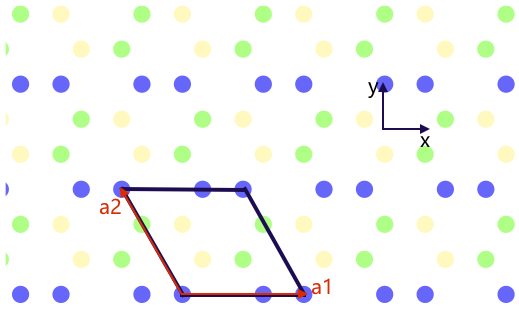
\includegraphics[width=0.6\linewidth]{problem1.png}
	\caption{Primitive vectors and primitive cells.}
	\label{fig:problem1}
\end{figure}
So in each unit cell, there are $2$ blue points, $2$ yellow points, $2$ green points. There are $6$ basis,
i.e.\ ,
$ \text{blue points} = \{\bm{0}, \frac{2}{3}\bm{a}_1 \}$;
$\text{green points} = \{\frac{2}{3}\bm{a}_1 + \frac{1}{3}\bm{a}_2, \frac{2}{3}\bm{a}_2 \}$;
$\text{yellow points} = \{ \frac{1}{3}\bm{a}_1 +\frac{1}{3} \bm{a}_2, \frac{1}{3}\bm{a}_1 + \frac{2}{3}\bm{a}_2\}$.


\section*{Problem \RMN{2}}
The primitive cell of \ce{NaCl} is plotted as Fig. \ref{fig:nacl}.
\begin{figure}[h]
	\centering
	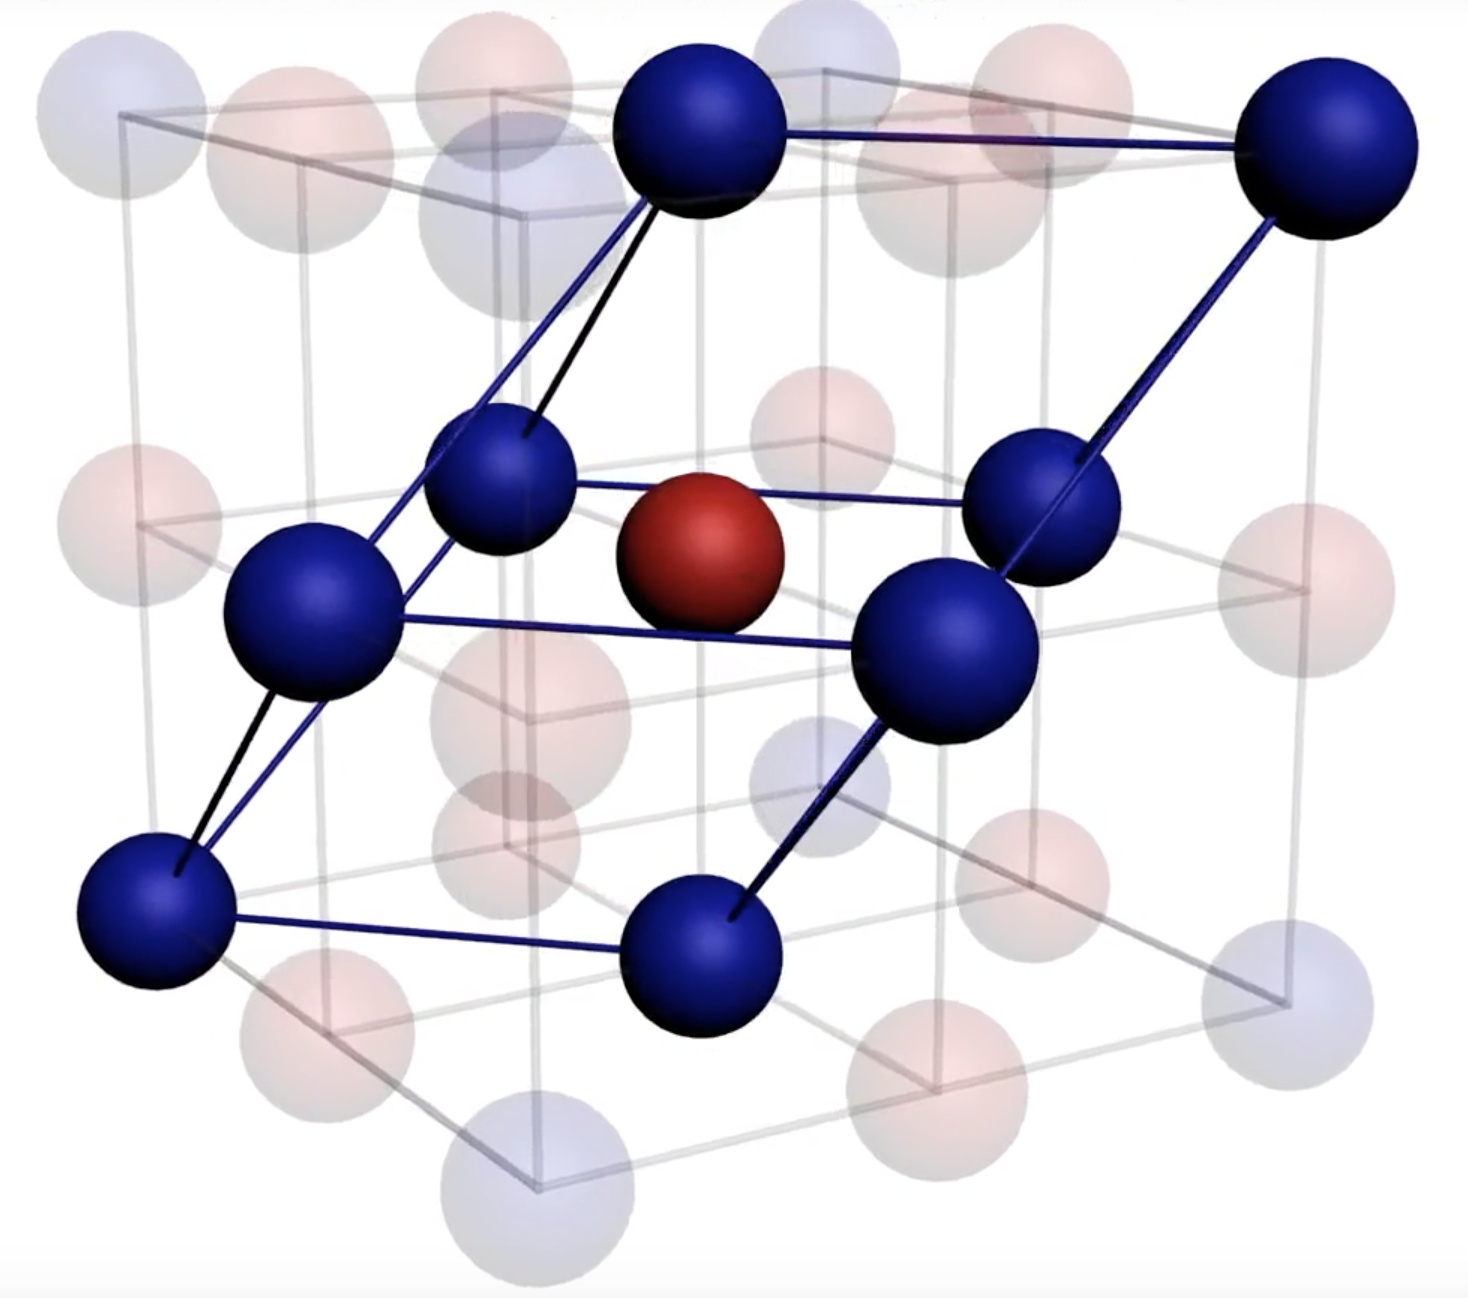
\includegraphics[width=0.4\linewidth]{nacl.png}
	\caption{Primitive cell of \ce{NaCl}.}
	\label{fig:nacl}
\end{figure}
Let 3D space directional vectors be $\hat{\bm{x}}$, $\hat{\bm{y}}$, $\hat{\bm{z}}$. Then
\begin{equation}
	\begin{cases}
		\bm{d}_1=\bm{0},                                   \\
		\bm{d}_2=\frac{a}{2}({\hat{\bm{x}}+\hat{\bm{y}}}), \\
		\bm{d}_3=\frac{a}{2}({\hat{\bm{x}}+\hat{\bm{z}}}), \\
		\bm{d}_4=\frac{a}{2}({\hat{\bm{y}}+\hat{\bm{z}}}).
	\end{cases}
\end{equation}
And primitive vectors are
\begin{equation}
	\begin{cases}
		\bm{a}_1=\frac{a}{2}({\hat{\bm{x}}+\hat{\bm{y}}}), \\
		\bm{a}_2=\frac{a}{2}({\hat{\bm{x}}+\hat{\bm{z}}}), \\
		\bm{a}_3=\frac{a}{2}({\hat{\bm{y}}+\hat{\bm{z}}}).
	\end{cases}
\end{equation}

So the primitive vectors of reciprocal lattice are
\begin{equation}
	\begin{cases}
		\bm{b}_1 =2\pi \frac{ \bm{a}_1 \times \bm{a}_3}{\bm{a}_1 \cdot \bm{a}_2 \times \bm{a}_3} =  \frac{2\pi}{a}\hat{\bm{x}}  + \frac{2\pi}{a}\hat{\bm{y}} - \frac{2\pi}{a}\hat{\bm{z}},  \\
		\bm{b}_2 = 2\pi\frac{\bm{a}_3 \times \bm{a}_1 }{\bm{a}_1 \cdot \bm{a}_2 \times \bm{a}_3} =   \frac{2\pi}{a}\hat{\bm{x}}  - \frac{2\pi}{a}\hat{\bm{y}} + \frac{2\pi}{a}\hat{\bm{z}}, \\
		\bm{b}_3 =2\pi \frac{\bm{a}_1 \times \bm{a}_2 }{\bm{a}_1 \cdot \bm{a}_2 \times \bm{a}_3} =  -\frac{2\pi}{a}\hat{\bm{x}}  + \frac{2\pi}{a}\hat{\bm{y}} + \frac{2\pi}{a}\hat{\bm{z}}. \\
	\end{cases}
\end{equation}


\section*{Problem \RMN{3}}
The primitive unit cell is encompassed by black lines, the primitive vectors are drawn by red lines,
2D space vectors are drawn aside. See Fig. \ref{fig:graphene}.
\begin{figure}[h]
	\centering
	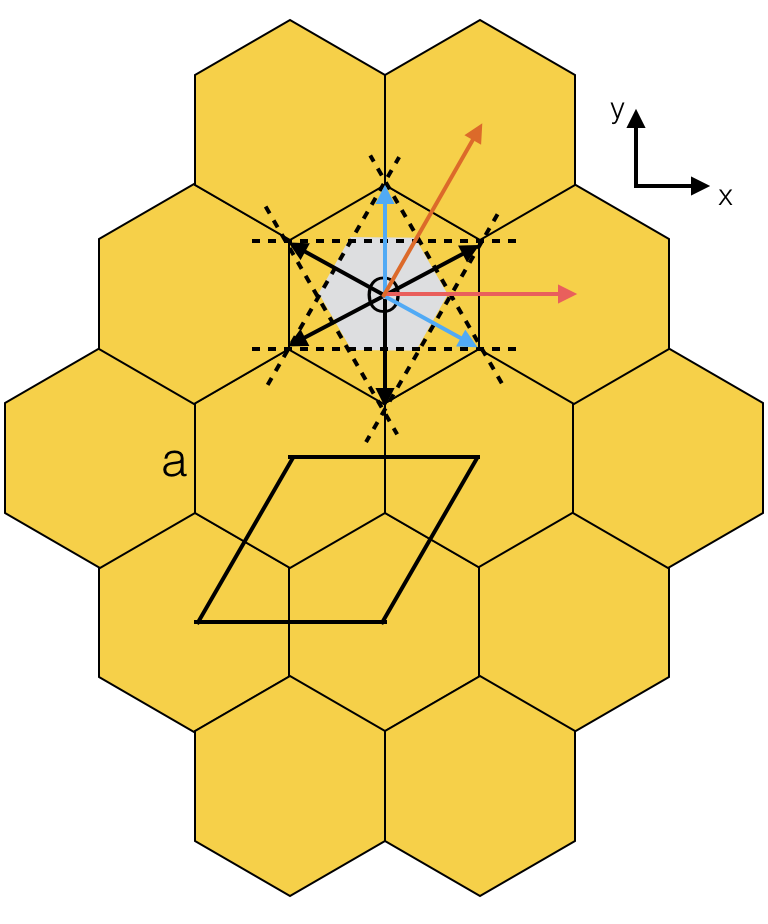
\includegraphics[width=0.4\linewidth]{graphene.png}
	\caption{Graphene's primitive cell.}
	\label{fig:graphene}
\end{figure}

So primitive vectors are
\begin{equation}
	\begin{cases}
		\bm{a}_1 = \sqrt{3}a \hat{\bm{x}},                                      \\
		\bm{a}_2 = \frac{\sqrt{3}}{2}a \hat{\bm{x}} + \frac{3}{2}a\hat{\bm{y}}.
	\end{cases}
\end{equation}
Since
\begin{equation}
	\bm{a}_i \cdot \bm{b}_j = 2\pi \delta_{ij},
\end{equation}
so the reciprocal primitive vectors are
\begin{equation}
	\begin{cases}
		\bm{b}_1 = \frac{2\pi}{\sqrt{3}a} \hat{\bm{x}} - \frac{2\pi}{3a} \hat{\bm{y}}, \\
		\bm{b}_2 = \frac{4\pi}{3a}\hat{\bm{y}}.
	\end{cases}
\end{equation}
It is clear that $\lvert \bm{b}_1 \rvert = \lvert \bm{b}_2 \rvert$.
Here the reciprocal primitive vectors are drawn in blue.
To sketch the first Brillouin Zone, simply select one lattice point, connect the nearest several points, and bisect those connections,
the intersection of these bisections would make the first Brillouin Zone.

So the gray area is the first Brillouin Zone.

\bibliographystyle{unsrt}
\bibliography{ref}
\end{document}
